\clearpage
% \section{Summary}
% In this supplement, we provide \textbf{(1)} human evaluation results and more ablation studies regarding the special tokens for knowledge graph linearization, \textbf{(2)} datasets and implementation details, \textbf{(3)} more explanations on baselines, and \textbf{(4)} additional qualtiative results.

\section{Additional experiments}
% \subsection{Experimental Results with LLAMA}
% Wednesday

\subsection{Additional Quantitative Analysis}
\label{sup_sec:aqa}
We also conduct experiments to verify the contribution of using $\texttt{[Rev]}$ to represent reverse relations and multiple consecutive tokens to represent each $\texttt{[Rev]}$ or $\texttt{[Int]}$ in Table~\ref{sup_tab:prompt}.
By adding \textbf{reverse tokens} to the knowledge, which allows mentioned entities that are tail entities in the provided triplets to be the starting points for the decoding, the performance is improved by 0.33 on BLEU-1 metric. 
Also, using \textbf{multiple consecutive tokens} to represent each $\texttt{[Rev]}$ or $\texttt{[Int]}$ (e.g., $\texttt{[Head]}$ $\Ent_1$ $\texttt{[Int{\textsubscript{\texttt{11}}}]}$ $\texttt{[Int{\textsubscript{\texttt{12}}}]}$ $\Rel_1$ $\texttt{[Int{\textsubscript{\texttt{21}}}]}$ $\texttt{[Int{\textsubscript{\texttt{22}}}]}$ $\Ent_{2}$ $\texttt{[Tail]}$) gives the performance gain on all the metrics since using the multiple tokens improve the capacity of representing the entities and the relations on top of language models.
By adding all the components, performance significantly improves by 0.56 on BLEU-1 metric compared to the linearized knowledge graph without any special tokens, which demonstrates the effectiveness of our proposed knowledge graph linearization approaches with special tokens. 
Interestingly, adding reverse tokens with using multiple consecutive tokens improves the overall performance compared to adding reverse tokens without using multiple consecutive tokens, which indicates that representing reverse relations is more effective when the capacity of the knowledge representation is increased. 
% Assume that the triplet $(e_1, r_1, e_2)$ is given.
% Given the triplet $(e_1, r_1, e_2)$, we can represent the triplet as $\texttt{[Head]} \ \Ent_2 \ \texttt{[Int{\textsubscript{\texttt{1}}}]} \ \Rel_1 \ \texttt{[Int{\textsubscript{\texttt{2}}}]}  \ \Ent_{1} \ \texttt{[Tail]}$ by adding the soft prompts $\texttt{[Head]},\texttt{[Int]},\texttt{[Tail]}$, which is corresponds to \textbf{Soft prompting}.
% % The base triplet representation is $\texttt{[Head]} \ \Ent_2 \ \texttt{[Int{\textsubscript{\texttt{1}}}]} \ \Rel_1 \ \texttt{[Int{\textsubscript{\texttt{2}}}]}  \ \Ent_{1} \ \texttt{[Tail]}$ without any reverse tokens.
% % By omitting soft prompts, we represent the triplet as $e_1, r_1, e_2$ for the input of the model.
% By adding \textbf{reverse tokens}, the triplets are represented as $\texttt{[Head]} \ \Ent_2 \ \texttt{[Rev{\textsubscript{\texttt{1}}}]} \ \Rel_1 \ \texttt{[Rev{\textsubscript{\texttt{2}}}]}  \ \Ent_{1} \ \texttt{[Tail]}$ when the given triplet $e_1, r_1, e_2$ satisfies the specific condition referred in Section 3.2 of the main paper.
% With multiple tokens of $\texttt{[Rev], [Int]}$, we represent the triplet as $\texttt{[Head]} \ \Ent_1 \ \texttt{[Int{\textsubscript{\texttt{11}}}]} \ \texttt{[Int{\textsubscript{\texttt{12}}}]} \ \Rel_1 \ \texttt{[Int{\textsubscript{\texttt{21}}}]}\texttt{[Int{\textsubscript{\texttt{22}}}]} \ \Ent_2  \ \texttt{[Tail]}$.
% The experimental results are in Table~\ref{sup_tab:prompt}.
% The table shows that all components of our prompting contribute to the improvement of the performance.  


\begin{table}[t]
    % \setlength{\tabcolsep}{0pt}    
    % \resizebox{\textwidth}{!}
    \small
    \centering
    
    \begin{tabular}{cc|ccccc}
        \toprule
	 Reverse & Multiple &   {B-1} & {B-2} & path@3\\
         \midrule 
         \midrule
            &            & 18.74&11.99&   {41.28}\\
        \checkmark &            & 19.07&12.03&  {44.54}\\
                   & \checkmark & 19.22&12.01&   {45.06}\\
        \checkmark & \checkmark & \textbf{19.30}&\textbf{12.10} &  \textbf{46.76}\\
        \bottomrule
    \end{tabular}
    \caption{Ablation studies on special tokens with OpenDialKG dataset. `Reverse' denotes reverse tokens and `Multiple' denotes multiple tokens.}
    \label{sup_tab:prompt}
\end{table}



\begin{table*}[t]
    \centering    
    % \setlength{\tabcolsep}{0pt}    
    \resizebox{\textwidth}{!}    
    {
    \begin{tabular}{llll}
        \toprule
          Dialog & Gold response & SURGE (Baseline) & DialogGSR (Ours) \\
         \midrule
         \midrule
         \begin{tabular}{@{}l@{}}
(a) Could you recommend and books by the author of\\ \quad \ \  Colour of Magic? \\
(b) The Colour of Magic has genre fantasy. So do you\\ \quad \ \  want to read fantasy books? \\
(a) Like Through  the Looking Glass?  Sure I like \\ \ \ \quad  Fantasy okay. \\
(b) yes like The Looking Glass Wars it's really a good \\ \quad \ \  book. I suggest reading it. \\
(a) Do you know who wrote it by any chance? \\
\end{tabular}
& 
         \begin{tabular}{@{}l@{}}
Yes Frank Beddor wrote it,\\ who also wrote Seeing Redd.
\end{tabular} & 
         \begin{tabular}{@{}l@{}}
Terry Pratchett
\end{tabular} &
\begin{tabular}{@{}l@{}}
It was written by \\Frank Beddor.
\end{tabular}\\         
    \midrule
        \multicolumn{4}{l}{\textit{\textbf{Knowledge triplets $\tau$ retrieved from Baseline}}} \\
        % & \multicolumn{3}{l}{\textit{\textbf{Knowledge triplets $\tau$ retrieved from GSR}}} \\
        \multicolumn{4}{l}{$\langle$ `The Colour of Magic', `written\_by', `Terry Pratchett' $\rangle$} \\
        % & \multicolumn{3}{l}{$\langle$ `Ashton Kutcher', `romantic relationship (with celebrities)', `Mila Kunis' $\rangle$}\\
        \multicolumn{4}{l}{$\langle$ `The Looking Glass Wars', `written\_by', `Frank Beddor' $\rangle$} \\
        % \multicolumn{4}{l}{$\langle$ `The Colour of Magic', `written\_by', `Terry Pratchett'$ \rangle$} \\
        % \multicolumn{3}{l}{$\langle$ `\colorbox{red}{Becca Fitzpatrick}', `write', `\colorbox{yellow}{Silence}'  $\rangle$}\\
        % \multicolumn{3}{l}{$\langle$ `\colorbox{yellow}{Silence}', `\colorbox{green}{released year}', `\colorbox{cyan}{2012}' $\rangle$}\\
        \midrule
        \multicolumn{4}{l}{\textit{\textbf{Knowledge triplets $\tau$ retrieved from DialogGSR}}}\\
        \multicolumn{4}{l}{$\langle$ `The Looking Glass Wars', `written\_by', `Frank Beddor' $\rangle$} \\
        \multicolumn{4}{l}{$\langle$ `Frank Beddor', `is-a', `Film Producer' $\rangle$} \\
        % \multicolumn{4}{l}{$\langle$ `Ashton Kutcher', `romantic relationship (with celebrities)', `Mila Kunis' $\rangle$}\\
        % \multicolumn{4}{l}{$\langle$ `Friends with Benefits', `starred\_actors', `Mila Kunis'  $\rangle$}\\
        % \multicolumn{4}{l}{$\langle$ `Friends with Benefits', `starred\_actors', `Patricia Clarkson' $\rangle$}\\
        \midrule
        \midrule
         \begin{tabular}{@{}l@{}}
(a) I like the book Where'd You Go, Bernadette. \\
\quad \ \ Do you have any other suggestions for me? \\
(b) Definitely!  That's a great book by Maria Semple.\\ \quad \ \   Do you like her? \\
(a) I do! Has she written anything else? \\
\end{tabular}
& 
         \begin{tabular}{@{}l@{}}
She is a screenwriter,\\ television producer, and\\ she produced Mad About You.

\end{tabular} & 
         \begin{tabular}{@{}l@{}}
She's written a lot \\of books, including \\Where'd You Go, Bernadette.\\ Have you read that one?
\end{tabular} &
\begin{tabular}{@{}l@{}}
She has. She also \\wrote the TV program,\\ Mad About You.\\ Have you heard of that one?
\end{tabular}\\         
    \midrule
        \multicolumn{4}{l}{\textit{\textbf{Knowledge triplets $\tau$ retrieved from Baseline}}} \\
        % & \multicolumn{3}{l}{\textit{\textbf{Knowledge triplets $\tau$ retrieved from GSR}}} \\
        \multicolumn{4}{l}{$\langle$ `Where'd You Go, Bernadette', `written\_by',	`Maria Semple' $\rangle$} \\
        % & \multicolumn{3}{l}{$\langle$ `Ashton Kutcher', `romantic relationship (with celebrities)', `Mila Kunis' $\rangle$}\\
        \multicolumn{4}{l}{$\langle$ `Where'd You Go, Bernadette',	`release\_year',	`2012' $\rangle$} \\
        \multicolumn{4}{l}{$\langle$ `2012',	`release\_year (reverse)',	`Where'd You Go, Bernadette' $\rangle$} \\
        \midrule
        \multicolumn{4}{l}{\textit{\textbf{Knowledge triplets $\tau$ retrieved from DialogGSR}}}\\
        \multicolumn{4}{l}{$\langle$ `Where'd You Go, Bernadette', `written\_by' ,`Maria Semple' $\rangle$} \\
        \multicolumn{4}{l}{$\langle$ `Maria Semple', `tv program produced', `Mad About You' $\rangle$} \\        
        \multicolumn{4}{l}{$\langle$ `Mad About You', `has\_genre', `sitcom' $\rangle$} \\
        % \multicolumn{4}{l}{$\langle$ `Ashton Kutcher', `romantic relationship (with celebrities)', `Mila Kunis' $\rangle$}\\
        % \multicolumn{4}{l}{$\langle$ `Friends with Benefits', `starred\_actors', `Mila Kunis'  $\rangle$}\\
        % \multicolumn{4}{l}{$\langle$ `Friends with Benefits', `starred\_actors', `Patricia Clarkson' $\rangle$}\\

        \midrule
        \midrule
         \begin{tabular}{@{}l@{}}
(a) Do you know any movies directed by \\ \quad \ \  Bennett Miller? \\
(b) He has some great ones. Have you seen \\ \quad \ \ Moneyball or Capote? \\
(a) I haven't seen Moneyball,\\ \quad \ \  who stars in it? \\
\end{tabular}
& 
         \begin{tabular}{@{}l@{}}
Steve Zaillian wrote Moneyball.\\ It starred Brad Pitt along with\\ Tammy Blanchard. It's a \\ really good movie!

\end{tabular} & 
         \begin{tabular}{@{}l@{}}
Capote stars Seymour\\ Hoffman and Ben\\ Stiller. It's a \\ romantic comedy.

\end{tabular} &
\begin{tabular}{@{}l@{}}
Tammy BLanchard and \\Brad  Pitt are in it. \\Do you like action movies?
\end{tabular}\\         
    \midrule
        \multicolumn{4}{l}{\textit{\textbf{Knowledge triplets $\tau$ retrieved from Baseline}}} \\
        % & \multicolumn{3}{l}{\textit{\textbf{Knowledge triplets $\tau$ retrieved from GSR}}} \\
        \multicolumn{4}{l}{$\langle$ `Moneyball', `starred\_actors', `Philip Seymour Hoffman' $\rangle$} \\
        % & \multicolumn{3}{l}{$\langle$ `Ashton Kutcher', `romantic relationship (with celebrities)', `Mila Kunis' $\rangle$}\\
        \multicolumn{4}{l}{$\langle$ `Capote', `starred\_actors',`Philip Seymour Hoffman' $\rangle$} \\
        \multicolumn{4}{l}{$\langle$ `Philip Seymour Hoffman', `starred\_actors (reverse)', `Moneyball' $\rangle$} \\
        \midrule
        \multicolumn{4}{l}{\textit{\textbf{Knowledge triplets $\tau$ retrieved from DialogGSR}}}\\
        \multicolumn{4}{l}{$\langle$ `Moneyball', `starred\_actors', `Tammy Blanchard' $\rangle$} \\
        \multicolumn{4}{l}{$\langle$ `Moneyball', `starred\_actors', `Brad Pitt' $\rangle$} \\        
        \multicolumn{4}{l}{$\langle$ `Moneyball', `starred\_actors', `Robin Wright' $\rangle$} \\
        % \multicolumn{4}{l}{$\langle$ `Ashton Kutcher', `romantic relationship (with celebrities)', `Mila Kunis' $\rangle$}\\
        % \multicolumn{4}{l}{$\langle$ `Friends with Benefits', `starred\_actors', `Mila Kunis'  $\rangle$}\\
        % \multicolumn{4}{l}{$\langle$ `Friends with Benefits', `starred\_actors', `Patricia Clarkson' $\rangle$}\\

        \midrule
        \midrule
         \begin{tabular}{@{}l@{}}
(a) Can you tell me some \\ \quad \ \  Beatrix Potter books? \\
(b) Would you prefer her biography,\\ \quad \ \  or children's literature? \\
(a) Children's literature please. \\
(b) Would you like The Tale of Peter \\ \quad \ \  Rabbit? Or The Tale of Mrs Tiggy-Winkle? \\ \quad \ \  I hear they're both good.\\
(a) Ill try Peter Rabbit,\\ \quad \ \  out of curiosity when \\ \quad \ \ were these books written? \\
\end{tabular}
& 
         \begin{tabular}{@{}l@{}}
I believe they were written \\ in the year 1905, to be exact.


\end{tabular} & 
         \begin{tabular}{@{}l@{}}
The Tale of Mrs. Tiggy-Winkle \\ was written in 1851.

\end{tabular} &
\begin{tabular}{@{}l@{}}
I'm not sure when they \\ were written, but they were\\ released in the year 1905.
\end{tabular}\\         
    \midrule
        \multicolumn{4}{l}{\textit{\textbf{Knowledge triplets $\tau$ retrieved from Baseline}}} \\
        % & \multicolumn{3}{l}{\textit{\textbf{Knowledge triplets $\tau$ retrieved from GSR}}} \\
        \multicolumn{4}{l}{$\langle$ `The Complete Tales of Beatrix Potter', `written\_by', `Beatrix Potter
' $\rangle$} \\
        % & \multicolumn{3}{l}{$\langle$ `Ashton Kutcher', `romantic relationship (with celebrities)', `Mila Kunis' $\rangle$}\\
        \multicolumn{4}{l}{$\langle$ `The Complete Adventures of Peter Rabbit', `written\_by', `Beatrix Potter
' $\rangle$} \\
        \multicolumn{4}{l}{$\langle$ `The Tale of Mrs. Tiggy-Winkle', `written\_by', `Beatrix Potter
' $\rangle$} \\
        \midrule
        \multicolumn{4}{l}{\textit{\textbf{Knowledge triplets $\tau$ retrieved from DialogGSR}}}\\
        \multicolumn{4}{l}{$\langle$ `The Tale of Mrs. Tiggy-Winkle', `written\_by', `Beatrix Potter' $\rangle$} \\
        \multicolumn{4}{l}{$\langle$ `The Tale of Mrs. Tiggy-Winkle', `release\_year', `1905' $\rangle$} \\        
        \multicolumn{4}{l}{$\langle$ `The Return Of Sherlock Holmes', `release\_year', `1905' $\rangle$} \\
      
    \bottomrule
    \end{tabular}
    }
    % \vspace{-2mm}
    \caption{\label{tab_sup:qual}Comparison on responses generated by SURGE~(Baseline) and DialogGSR given a dialog.}
\end{table*}

\subsection{Additional Qualitative Analysis}
\label{supp:add_qual}
In Table~\ref{tab_sup:qual}, we provide additional qualitative examples for what we have shown in Table~\ref{tab:qual} of the main paper.
Our DialogGSR often generates high-quality responses similar to the main paper.
For example, in the first example, our DialogGSR generates a factually correct response "It was written by Frank Beddor" based on the retrieved triplet $\langle$`The Looking Glass Wars', `written\_by', `Frank Beddor'$\rangle$ while SURGE generates a factually incorrect response "Terry Pratchett" with the same triplet $\langle$`The Looking Glass Wars', `written\_by', `Frank Beddor'$\rangle$.
It demonstrates that our DialogGSR is more effective in generating responses even with the same knowledge information given. 
In the second example, DialogGSR successfully generates a factually correct response by retrieving context-relevant knowledge triplets whereas the factually incorrect response is generated by the baseline due to the retrieval of irrelevant knowledge.
These results demonstrate that our generative retrieval is effective in retrieving informative knowledge and generating knowledge-grounded dialogs.
% In particular, our DialogGSR shows better response quality than the baseline as the number of turns is larger as seen in the table, which demonstrates the effectiveness of our approach for dealing with information bottleneck issues.

\section{Experimental details}
\label{supp:exp_details}
% \subsection{Datasets}
% \label{supp:datasets}
% \textbf{OpenDialKG}\footnote{Licensed under CC-BY-NC-4.0} is an open-domain dialog dataset that consists of 15K dialogs with 91K turns and 1.12M triplets from Freebase~\cite{bast2014easy} knowledge graph.
% The knowledge graph has 1,190,658 triplets, 100,813 entities, and 1,358 relations.
% There are 49\% of the turns having gold knowledge triplets.
% Following \cite{galetzka2020corpus}, we randomly split the dialogs into train~(70\%), validation~(15\%), and test~(15\%) sets.
% With OpenDialKG dataset, we evaluate the response generation and retrieval performance of our DialogGSR with other baselines following \cite{kang2022knowledge,tuan2022towards}.
% The baseline results in Table 1 of the main paper are reported from \cite{kang2022knowledge}.

% \textbf{KOMODIS}\footnote{Copyright (c) 2020 Fabian Galetzka, Licensed under MIT license} is a closed-domain dialog dataset that consists of 7.5k dialogs with 103k turns and the corresponding KG, which contains 88K triplets.
% Following \cite{moon2019opendialkg,kang2022knowledge,galetzka2020corpus}, we randomly split the dialogs into train~(70\%), validation~(15\%), and test~(15\%) sets for KOMODIS dataset.
% With KOMODIS dataset, we evaluate the response generation performance of our DialogGSR with other baselines following \cite{kang2022knowledge,galetzka2021space}.
% The baseline results in Table 2 of the main paper are reported from \cite{kang2022knowledge}.

\subsection{Implementation details}
In this section, we describe the implementation details not included in our main paper.
For all the experiments, we use PyTorch\footnote{Copyright (c) 2016-Facebook, Inc (Adam Paszke), Licensed under BSD-style license}~\cite{paszke2019pytorch} and Transformer module of Huggingface\footnote{Copyright 2018-The Hugging Face team, Licensed under the Apache license}~\cite{wolf2019huggingface} as our code base.
All experiments are conducted with 48GB NVIDIA RTX A6000 GPU.
We select the best model on the validation set to evaluate the performance of all experiments.
The epoch for training is set to 50 and the weight decay is 0.1. 
We use AdamW optimizer~\cite{Loshchilov2019adamw} to train our model and adopt learning rate decay.
\paragraph{Knowledge graph{\textendash}constrained decoding.}
Without the graph constraints, the language model is prone to generate invalid or irrelevant subgraphs due to the language model's bias~\cite{chen2022relation,de2021autoregressive}.
To inject the knowledge graph information into the language model in the decoding step, we present a knowledge graph{\textendash}constrained decoding method.
% The $\text{TopK-Select}(\cdot)$ function of the algorithm selects Top-$k$ candidates from all candidates $w \in \mathcal{V}$ by calculating $\log\tilde{p}\left(w|\boldsymbol{x}, \boldsymbol{y}_{<t}^{\left(i\right)}\right)+ \log \tilde{p}\left(\boldsymbol{y}_{<t}^{\left(i\right)}|\boldsymbol{x}\right)$.  
We use $\alpha=0.8$ and $k=2$ for calculating Katz~\cite{katz1953new} index-based entity informativeness score.
$p_{\text{graph}}$ is defined in Eq.~\eqref{eq:katz} of the main paper, and $b$ is 5.

% \paragraph{Evaluation metrics}
% We evaluate the dialog generation performance of different models with BLEU~\cite{papineni2002bleu}, ROUGE~\cite{lin2004rouge}, and unigram F1 score, by comparing the generated responses with the gold responses.
% In addition, we use the KQA metric~\cite{kang2022knowledge}, which measures whether the factually correct and necessary knowledge is contained in the generated response given the dialog history. 
% % The baseline results are reported from \citet{kang2022knowledge}.
% We also evaluate the performance of the retriever with path@k metrics, which are the recall@k of ground-truth paths following \cite{moon2019opendialkg,jung2020attnio}.

\section{Details of Human Evaluation}
\label{sec:human_evaluation_detail}

We first randomly selected 30 dialogs from OpenDialKG test dataset~\cite{moon2019opendialkg} and generated responses using our model and SURGE~\cite{kang2022knowledge} for the comparison.
We recruited 22 participants who were not involved in our research and allowed the use of external sources, such as the Internet, to verify the factual correctness of generated responses. 
Following the process outlined in the other work~\cite{kang2022knowledge}, we utilized a 3-point Likert-like scale to evaluate three criteria: Consistency, Informativeness, and Fluency. 
\textbf{Consistency} measures the coherence and logical flow within the context of the conversation, \textbf{Informativeness} assesses the correctness and usefulness of the information in the generated responses, and \textbf{Fluency} focuses on the naturalness and linguistic quality of the dialog. 
With the human evaluation metrics and the automatic metrics in the main paper, we establish a comprehensive evaluation framework that enables accurate comparisons between models, enhancing the reliability of our assessment.


\begin{figure}

\centering
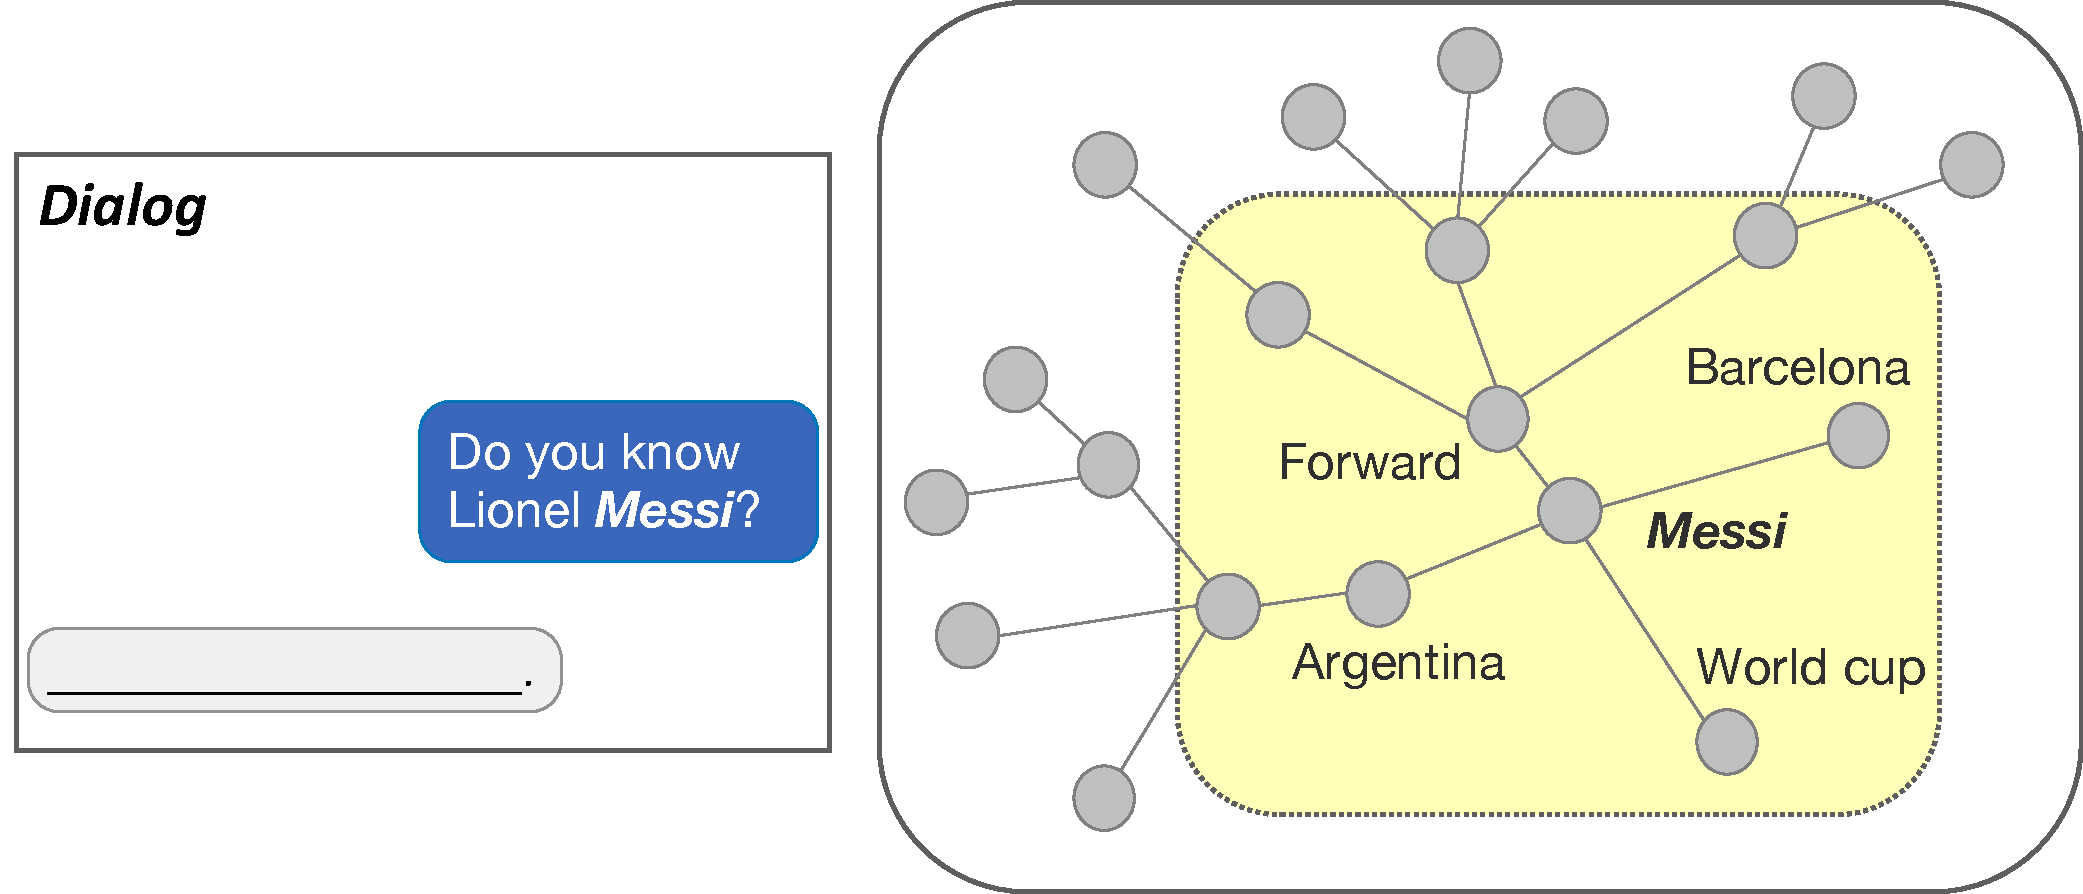
\includegraphics[width=1.0\linewidth]{Figures/subgraph.pdf}
\caption{An example of extracting a 2-hop candidate subgraph from the knowledge graph. Yellow region indicates the 2-hop candidate subgraph centered on the mentioned entity ``Messi".}
\label{fig:subgraph}
\end{figure}

\section{Baselines}
\label{supp:baselines}
\subsection{Response Generation}
In our experiments, the following baseline models are used for comparing the response generation performance with our DialogGSR.

\begin{itemize}
    \item \textbf{T5{\textendash}small~(w/o KGs)}\footnote{Licensed under the Apache license}~\cite{roberts2019exploring}: T5-small is an encoder-decoder Transformer architecture for various natural language processing tasks.
    \item \textbf{Space Efficient (series)}\footnote{Copyright (c) 2021 Fabian Galetzka, Licensed under MIT license}~\cite{galetzka2021space}: Space Efficient (series) is the model proposed in \cite{galetzka2021space}. It utilizes all knowledge triplets related to the entities by matching the entities of KG and the entities mentioned in dialog history without any retrieval process.
    This model sequentially encodes knowledge triplets and feeds them into the encoder.
    \item \textbf{Space Efficient (parallel)}~\cite{galetzka2021space} : This model is also proposed by \cite{galetzka2021space}. Different from Space Efficient (series), this model constructs a segmentation block for each entity and encodes the relation in the segmentation block to reflect relational information.
    \item \textbf{Diff-KG}~\cite{tuan2022towards}: Diff-KG reasons differentiable knowledge paths to jointly generate a response with the dialog history.
    After the path reasoning, entities included in the path are concatenated with dialog history, and they are fed into a pretrained language model. 
    \item \textbf{SURGE (unsup.)}~\cite{kang2022knowledge}: SURGE is a graph neural network{\textendash}augmented Transformer-based dialog generation model that encodes knowledge triplets with graph neural networks.
    SURGE also retrieves context-relevant triplets via a subgraph retriever.
    This model trains the retriever without the guidance of gold knowledge and is implicitly trained with response generation loss.
    \item \textbf{SURGE (semi-sup.)}~\cite{kang2022knowledge}: SURGE (semi-sup.) uses gold knowledge to train the retriever. 
    \item \textbf{SURGE (contrastive)}~\cite{kang2022knowledge}: SURGE (contrastive) uses both the retrieval supervision from SURGE (Semi-sup.) and contrastive learning to encourage the encoder output and the decoder output to be closer.
\end{itemize}
% \textbf{T5~(w/o KG)}~\cite{roberts2019exploring} is a fine-tuned T5 model without using the knowledge graph.
% \textbf{Space Efficient}~\cite{galetzka2021space} generates dialogs with dense representation of knowledge graph with two encoding methods: \textbf{Space Efficient~(series)} and \textbf{Space Efficient~(parallel)}.
% \textbf{EARL}~\cite{zhou2021earl} is the latest RNN{\textendash}based model on knowledge-grounded dialog system.
% \textbf{Diff-KG}~\cite{tuan2022towards} is a model that retrieves knowledge triplets with differentiable path traversal on KG when generating responses. 
% \textbf{SURGE}~\cite{kang2022knowledge} is a GNN-based dialog generation model that encodes knowledge triplets with GNNs.
% \textbf{SURGE~(unsup.)} trains subgraph retriever without supervision on gold knowledge and implicitly learns to select gold knowledge and \textbf{SURGE~(semi-sup.)} uses gold knowledge to guide the subgraph retriever for selecting context-relevant knowledge.

\subsection{Knowledge Retrieval}
% We take nine models following \cite{tuan2022towards} as baselines including DiffKG~\cite{tuan2022towards} and SURGE~\cite{kang2022knowledge}, which are already introduced.
% Other seven models are Seq2Seq, Extended Encoder-Decoder~\cite{parthasarathi2018extending}, Tri-LSTM~\cite{young2017augmenting}, DialKG Walker~\cite{moon2019opendialkg}, AttnFlow~\cite{jung2020attnio}, and AttnIO~\cite{jung2020attnio}.
% DialKG Walker~\cite{moon2019opendialkg}.
% Different from our DialogGSR, DiffKG, and SURGE, these seven methods are designed only for knowledge retrieval task.
The models below are used as the baselines for validating the effectiveness of our DialogGSR on knowledge subgraph retrieval.

\begin{itemize}
    \item \textbf{Seq2Seq}~\cite{sutskever2014sequence}: Seq2Seq is used as a baseline in \cite{moon2019opendialkg,tuan2022towards}. Given all of the dialog contexts, Seq2Seq generates entity paths.
    \item \textbf{Tri-LSTM}~\cite{young2017augmenting}: Tri-LSTM is another baseline in \cite{moon2019opendialkg,tuan2022towards}. It encodes dialog contexts and related 1-hop knowledge from a KG to retrieve knowledge paths. 
    \item \textbf{Ext-ED (Extended Encoder-Decoder)}~\cite{parthasarathi2018extending}: Extended Encoder-Decoder is also one of the baselines in \cite{moon2019opendialkg,tuan2022towards}. 
    It generates a response conditioned on an external knowledge vector input, which is encoded by GloVe embedding.
    \item \textbf{DialKG Walker}~\cite{moon2019opendialkg}: DialKG Walker is an attention-based knowledge path retrieval model designed to traverse a knowledge graph with dialog context and knowledge paths.
    \item \textbf{AttnFlow}~\cite{jung2020attnio}: AttnFlow is an attention-based knowledge path retrieval model based on GAT~\cite{velivckovic2018graph} and the encoded dialog context.
    It only uses incoming attention flow to update knowledge representation.
    \item \textbf{AttnIO}~\cite{jung2020attnio}: AttnIO is an extension of AttnFlow, where both incoming and outcoming attention flows are used to represent knowledge paths with dialog contexts and entity features.
\end{itemize}

% \subsection{Knowledge graph prompt.}
% We shortly explain the baselines used in Table 5 of the main paper.
% \begin{itemize}
%     \item \textbf{Pre-defined}: We manually generate prompts for the 10 most frequent relations found in OpenDialKG (ex. \texttt{has\_genre} $\rightarrow$ \texttt{has a genre of}). 
%     This manual generation process accounts for 30.1\% of all triples and the remaining triplets are not converted. 
%     \item \textbf{Mine}~\cite{jiang2020can}: Mine proposes mining techniques and applies them to the T-REx subset datasets\footnote{Copyright (c) 2017 hady elsahar, Licensed under MIT license}~\cite{elsahar2018t} to generate prompts.
%     The mining process generates multiple prompts for each specific relation $r$, and we select the prompt with the highest weight.
%     % The prompt has a set of 41 relations obtained from Wikidata.
%     \item \textbf{\textit{full-rel2text}\footnote{Copyright 2022 Zdeněk Kasner, Licensed under the Apache license}}~\cite{kasner2023mind}: REL2TEXT\footnote{https://github.com/kasnerz/rel2text} is a data-to-text model, which converts knowledge triplets to the corresponding sentences.
%     We utilize an off-the-shelf model trained with the REL2TEXT dataset to generate full sentences for all our triples.
% \end{itemize}
% \textcolor{blue}{
% In Table 5 of the main paper, we present an analysis of our proposed knowledge graph soft prompting, comparing it to three existing data-to-text approaches. 
% First, for human-annotated pre-defined prompts, we manually generate prompts for the 10 most frequent relations found in OpenDialKG (ex. \texttt{has\_genre} $\rightarrow$ \texttt{has a genre of}). 
% This manual generation process accounts for 30.1\% of all triples.
% Second, Mine~\cite{jiang2020can} generated prompts through mining techniques applied to the T-REx subset dataset\footnote{Copyright (c) 2017 hady elsahar, Licensed under MIT license}~\cite{elsahar2018t}, which has a set set of 41 relations obtained from Wikidata. 
% the mining process generates multiple prompts for each specific relation $r$, and we select the prompt with the highest weight. 
% We conducted experiments with data that strictly overlapped our own dataset among the generated triple-prompt pairs.
% Finally, \textit{full-rel2text}\footnote{Copyright 2022 Zdeněk Kasner, Licensed under the Apache license}~\cite{kasner2023mind} created a new dataset called REL2TEXT\footnote{https://github.com/kasnerz/rel2text} which can help to replace the hand-crafted templates on downstream tasks.
% We utilize a model trained on the REL2TEXT dataset to generate full sentences for all our triples.
% }

% \textbf{KPDG~(w/o full KG)} learns knowledge path retriever without using full knowledge graphs 
% more details of experimental setup and baselines are discussed in the appendix.
% \section{Discussion}
% \section{Potential Risks}
% DialogGSR is a knowledge graph{\textendash}grounded dialog generation model for generating responses with autoregressively retrieved knowledge graphs.
% We think that this paper does not have any direct negative societal impacts. 
% However, similar to other dialog generation methods, DialogGSR can be applied to malicious applications.  
% Dialog generation models can manipulate factual information and then generate factually wrong responses. 
% Also, dialog generation models may generate biased responses that are learned from opinionated news and posts online.
% Especially responses on politics, religions, and diplomacy require precautions.
% % \textcolor{red}{It is also applied to generate unknowable information such as political opinions, religions, and search engines.}
% To address these societal issues, benchmark datasets without containing any private information should be released, and the methods that detect the source of texts need to be further studied.

% \subsection{Limitations}
% DialogGSR generatively retrieves token sequences of the subgraph from the knowledge graph and then generates a response with the retrieved subgraph.
% However, similar to works using graph retrieval on knowledge-grounded dialog generation, our generative subgraph retrieval retrieves only the knowledge contained in the knowledge graph.
% Second, the benchmark dataset for knowledge graph{\textendash}grounded dialog generation is limited.
% Except for OpendialKG~\cite{moon2019opendialkg} dataset, there is no dataset on dialog generation with a large-scale knowledge graph.
% So, new benchmark datasets on dialog generation with knowledge graphs deserve more attention.

% \input{Tables/prompt_table}